\chapter{Programming - Saw Parameters Screen}
\section{Overview}\paragraph*{The}\textbf{Programming - Saw Parameters} screen (Figure 7.1) provides the Operator programming access to the \textbf{Saw Operation Parameters} used while in \textit{Auto} mode. The Operator is able to make immediately initiated changes to the \textit{Cut Depth} the \textit{Blade Kerf} and the \textit{Motor Current Target}. Navigation is possible to the main \textbf{Manual} screen, the \textbf{Block Program} screen, both the \textbf{Vertical Axis} and \textbf{Cross Travel Axis} manual screens, and of course the \textbf{Main} operation screen. There is also an indicator for the Cross Travel Global Speed Override enabled state.
\begin{figure}
	\centering
	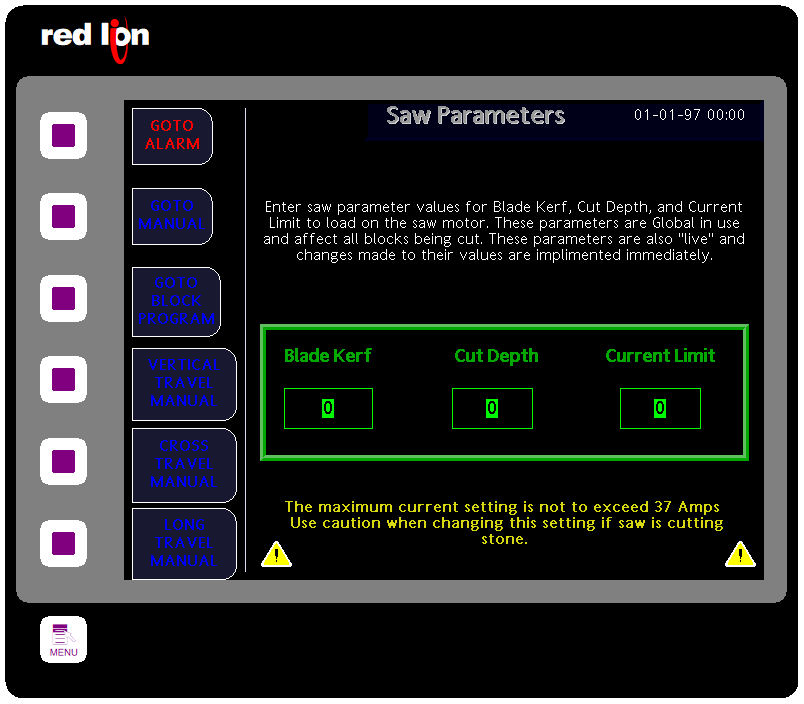
\includegraphics[width=0.5\linewidth]{screen-captures/program/pgm-saw-info}
	\caption{Programming - Saw Parameters Screen}
	\label{fig:prg-saw-param}
\end{figure}
\section{Details}\paragraph*{The}\textbf{Saw Parameters} screen details are divided into the following categories ...
\begin{list}{$\diamond$}{}
	\item \textbf{Screen Navigation}
	\item \textbf{Parameters}
	\item \textbf{Cross Travel Speed Override State}
\end{list}
\pagebreak
\subsection{Screen Navigation}
\paragraph*{Is}performed by using the programmable Function Keys (FKeys) located down the left hand side of the OI Terminal (refer to Figure 7.2). The Operator may navigate to the following screens ...
\begin{list}{$\diamond$}{}
	\item \textbf{GOTO Alarm} Navigate to Alarm Screen.
	\item \textbf{GOTO MANUAL} Navigate to Main Manual Screen.
	\item \textbf{GOTO BLOCK PROGRAM} Navigate to Block Program Screen.
	\item \textbf{VERTICAL MANUAL} Navigate to Vertical Manual Control Screen.
	\item \textbf{CROSS TRAVEL MANUAL} Navigate to Cross Travel Manual Control Screen.
	\item \textbf{LONG AXIS MANUAL} Navigate to the Long Axis Manual Control Screen.
\end{list}
\begin{figure}
	\centering
	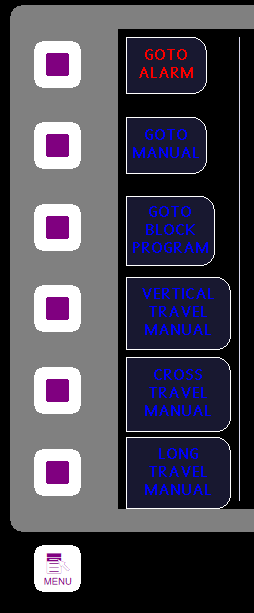
\includegraphics[width=0.2\linewidth]{screen-captures/program/pgm-saw-info-nav}
	\caption{Saw Parameter Screen Navigation}
	\label{fig:pgm-saw-info-screen-nav}
\end{figure}
\paragraph{\textbf{\LARGE \textcolor{blue}{i}}}
The Menu Key located on the terminal at the lower left below the FKey's, will return the Operator to the Main Screen, from all other screens.\\
\begin{minipage}{4cm}
	\begin{picture}(20,70)
		
\includegraphics[width=.5\linewidth]{screen-captures/menu}
	\end{picture}
\end{minipage}\begin{minipage}[]{11cm}
	\paragraph{\textbf{\LARGE \textcolor{blue}{i}}} The Menu Key is pictured as it looks on the Terminal.
\end{minipage}
\pagebreak
\subsection{Saw Parameters}\paragraph*{Parameters}are "live" settings that take affect immediately after changing them. The Operator should exercise caution when changing them while running automatically. The \textbf{\textit{Blade Kerf}} can be set to an accuracy of one thousandths of an inch by the Operator. The \textbf{\textit{Target Current}} while cutting can be set within the stated limits specified on screen. Down to a tenth of an ampere in resolution. The \textbf{\textit{Cut Depth}} can be set to any amount depending on Operator requirements, even decimal inches.
\begin{figure}
	\centering
	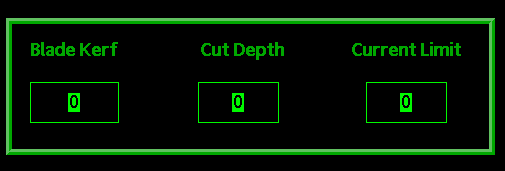
\includegraphics[width=.2\linewidth]{screen-captures/program/pgm-saw-info-entry}
	\caption{Saw Parameter Entry Fields}
	\label{fig:pgm-saw-info-entry}
\end{figure}
\paragraph{\textbf{\LARGE \textcolor{blue}{i}}}The Operator should exercise caution when changing these parameters while running in auto mode. The change will be applied immediately. It is especially important when adjusting cut depth, not to make too aggressive of a drop amount.
\subsection{Cross Travel Speed Override State}\paragraph*{Cross Travel Speed Override State}is an indicator that shows whether the \textbf{\textit{Cross Travel Speed Override}} is in an enabled or disabled state. When the override is enabled the indicator will be "lit" and will have the word \textbf{On} instead of \textbf{Off}. The actual enabling and speed setting is accessed through the \textbf{\textit{Program Check Screen}}. 
\begin{figure}
	\centering
	
\includegraphics[width=.2\linewidth]{screen-captures/program/pgm-cross-travel-spd-or}
	\caption{Saw Parameter Entry Fields}
	\label{fig:pgm-cross-travel-spd-or}
\end{figure}
\paragraph{\textbf{\LARGE \textcolor{blue}{i}}}The Operator can use this indicator to quickly see if the saw has the speed override enabled.
